%!TEX root = ../report.tex
\section{Leistungsdiagnostik}
Leistungsdiagnostik ist die Feststellung der Wettkampfleistung, von Wettkampf-Teilleistungen und von Leistungsvoraussetzungen.
Die Messung der Leistungsvorraussetzungen erfolgt über motorische Tests, leistungsphysiologische Verfahren (Laktat), biomechanische Verfahren (Laufanalysen) und psychologische Verfahren.
Die Messung der Wettkampfleistung über biomechanische Messungen (von einzelnen Läufen), Wettkampfdokumentationen und Spielbeobachtungen.

\subsection{Theoretische vs.\ Praktische Leistungsdiagnostik}
\paragraph{Theoretische Leistungsdiagnostik (TLD)}
Leistungsdiagnostik zum Zweck der Erstellung allgemeiner Aussagen über die Leistungsstruktur einer Sportart.\\
Typische TLD Fragestellungen:
\begin{itemize}
  \item Allgemeine Modellierung der sportlichen Leistung
  \item Sportartspezifische Modellbildung
  \item Alters- und Geschlechtsabhängigkeit der Leistungsstruktur
  \item Abhängigkeit der Leistungsstruktur vom Leistungsniveau
  \item Erstellung statistischer Normen
\end{itemize}
\paragraph{Praktische Leistungsdiagnostik (PLD)}
Leistungsdiagnostik im Kontext eines Trainingsprozesses.
PLD diagnostiziert die Wettkampfleistung und den Leistungszustand von Mannschaften und Athleten.
PLD ergängzt die Methoden von TLD mit qualitativen Analyzen von Einzelfällen.
Die Unterschiede von TLD und PLD liegen vorallem darin, dass sich PLD eher mit Einzelfällen und TLD eher für allgemeine, statistische Aussagen interessiert.
Die beiden Methoden beeinflussen sich allerdings: TLD generiert Hintergrundwissen für PLD und PLD liefert die VOrgaben für TLD (Hypothesen, Inspiration für Modelle).

\subsection{Leistungsdiagnostik in Sportspielen}
Sportspiele sind Sportarten mit international kodifiziertem Regelwerk, bei denen zwei Parteien in einen Interaktionsprozess eintreten, der dadurch zustande kommt, dass beide Parteien gleichzeitig ihr eigenes Spielziel anstreben und verhindern wollen, dass die gegnerische Partei ihr Spielziel erreicht; das Spielziel in den Sportspielen ist eine in den Regeln festgelegte, symbolische Handlung.
\paragraph{Problem} Das sichtbare Verhalten in Sportspielen lässt nicht direkt auf die zugrundeliegenden Leistungsvoraussetztungen schließen.
Außerdem ist das Verhalten dynamisch, d.h.\ zeitlich vergänglich, was Modellierung schwieriger macht.
\paragraph{Dynamische Systemtheorie} Klasse von Modellen, mit denen versucht wird, die Komplexität, Veränderungen in der Zeit (Dynamik) und interne Wechselwirkungen von Systemen abzubilden.\\
Grundbegriffe:\\
\begin{itemize}
  \item Zustandsraum: Menge der Zustände, die ein System einnehmen kann
  \item Attraktoren: Häufig aufgesuchte Punkte in einem Zustandsraum, Punkte mit Anziehungskraft
  \item Kontrollparameter: Variablen, die das System durch den Zustandsraum treiben
  \item Systemdynamik: Beschreibung des Systemverhaltens in der Zeit
\end{itemize}
\paragraph{Markov-Ketten Modellierung} bringt eine gute Beschreibung in vielen Sportspielen und hat eine gute Anwendung in Simulationen der TLD.\@
\paragraph{Random-Walk Modellierung}
In vielen Spielsportarten haben wir alternierenden Ballbesitz (Handball, Basketball, Fussball?).
Der Ballbesitz endet entweder mit Tor oder Kein Tor: Zufallsexperiment.
Eine Folge von Zufallsexperimenten, deren Ergebnisse aufaddiert werden, nennt man einen Random Walk.
Ein Handballspiel kann modelliert werden als zwei parallel laufende Random Walks.\\
\textbf{Modellierung:}\\
\begin{enumerate}[nolistsep,noitemsep]
  \vspace{-1em}
  \item Berechne die momentane Spielstärke mit einem Moving Average über 4 Moving Averages über den Erfolg in 4 Ballbesitzen
  \item Vergleiche die momentane Spielstärke der beiden Mannschaften: unabhängiger, positiv (direkt proportionaler) oder negativer (indirekt proportionaler) Zusammenhang
  \item Berechne die momentane Korrelation zwischen den beiden momentanen Spielstärken und überprüfe die Ergebnisse aus 2.
\end{enumerate}
Problem: Korrelation nicht über das ganze Spiel gleich.
Lösung: moving correlation.
\paragraph{Perturbation} ``Störung'' des relativen Gleichgewichts in einem Ballwechsel,
geht einem Punktgewinn voraus.

\subsection{Spielanalyse}
Spielanalyse ist die analytische, zielgerichtet Untersuchung eines Sportspiels zum Zweck der Leistungsdiagnose.
Teilbereiche sind die Eigenanalyse, Gegneranalyse und Spielstrategieanalysen.
Ablauf einer Spielanalyse:
\begin{enumerate}
  \item Aus der Spielanalyse wird eine Antizipation des Aufeinandertreffens entwickelt
  \item Daraus erfolt eine Strategiewahl
  \item Die Strategie wird mit unter Umständen kurzfristigen Änderungen umgesetzt, woraus wieder eine Spielanalyse erstellt werden kann.
\end{enumerate}
\paragraph{Prinzipielle Probleme}
\begin{itemize}
  \item Praktische Spielanalyse ist grundsätzlich nicht algorithmisch-quantitativ
    \begin{itemize}
      \item Alles hängt mit allem Zusammen!
      \item kleine Stichproben, Einzelfälle!
      \item Erkenntnislogik der Inferenzstatistik hilft nicht weiter
      \item Deskriptive Statistik als Hinweisgeber
    \end{itemize}
  \item Eher qualitative Argumentationslogik
    \begin{itemize}
      \item Ganzheitliche Analyse und Interpretation von Spielhandlungen
      \item Hintergrundwissen über Einzelfall
      \item Validität der Analyse entsteht über rationales Argumentieren
      \item Perspektive und Rückmeldung der Spieler
    \end{itemize}
\end{itemize}
\paragraph{Methodik}
Entwicklung von Spilerprofilen:
\begin{itemize}
  \item Skill-Profil: technisch-taktisches Repertoire
  \item Intra-Rally-Profil: Verhaltensabhängigkeit von der räumlichen Konstellation im Ballwechsel
  \item Inter-Rally-Profil: Verhaltensabhängigkeit vom zeitlichen Kontext des Ballwechsels
  \item Team-Profil: Verhaltensabhängigkeit vom gegnerischen Team
\end{itemize}
Analyseschritte zur Profilsuche:
\begin{enumerate}
  \item Filterung: Auswahl von Ballwechseln und Spielsituationen\\
    Filterstrategien: nach bestimmten Konstellationen suchen, nach Ergebnis suchen
  \item Quantitative Voranalyse: Suche nach quantitativen Verhaltensauffälligkeiten
    Beschreiben taktisch relevanten Spielverhaltens
  \item Qualitative Hauptanalyse: Analyse des Videomaterials und Ableitung von Konsequenzen.
    \begin{enumerate}
      \item Gegneranalyse: Anhand der Videos überprüfen ob die quantitativen Auffälligkeiten wirklich auf den Klassifikator zurückzuführen sind.
      \item Strategieentwicklung: Matchplan, Zustandsplan, Situationsplan
    \end{enumerate}
\end{enumerate}
\begin{figure}[H]
  \centering
  \caption{Zweck von Beobachtungssystemen}
  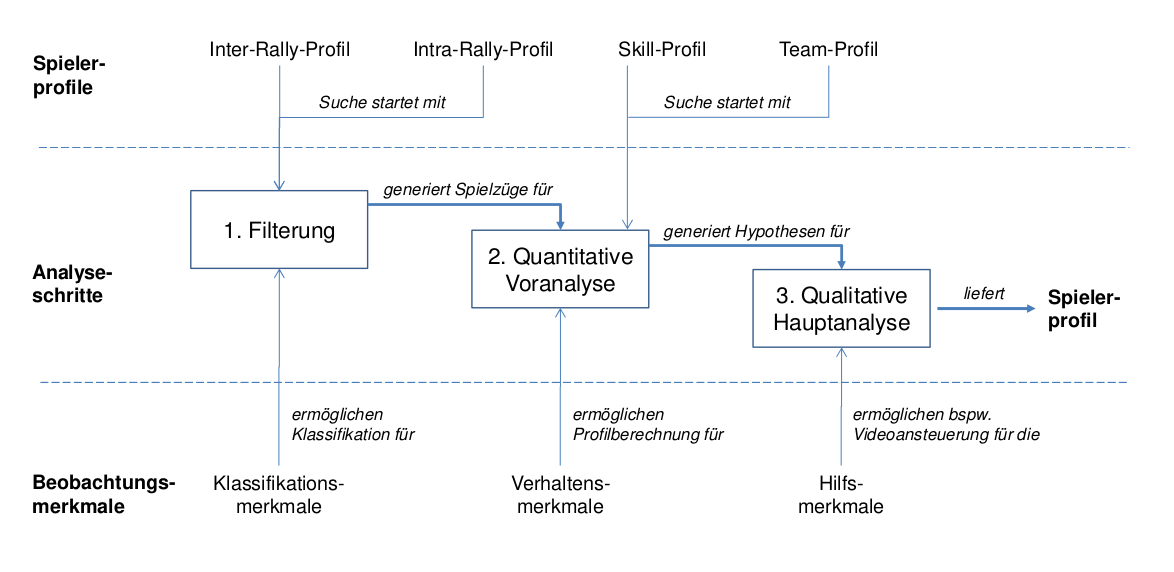
\includegraphics[width=.7\textwidth]{pictures/leistungsdiagnostik_beobachtungssystem_zweck.png}
\end{figure}
\paragraph{Softwareunterstützung}
Klassischer Funktionsumfang:
\begin{itemize}
  \item Kopplung von Videoplayer mit Datenbank
  \item Markieren von Videopositionen
  \item Zuordnung von Merkmalen zu Videopositionen
  \item Filtern von Videoszenen auf Basis der Merkmale
  \item Einfache Statistiken und Visualisierungen
\end{itemize}
\paragraph{psychosoziale Aspekte}
\begin{itemize}
  \item Analyse ist nicht ergebnissoffen: Suchen nach Hinweisen für das, was man eh schon glaubt zu wissen.
  \item Trainermeinung wird Athleten ``aufgedrückt'': Beteiligung der Athleten, Konsens schaffen!
  \item Instrumentalisierung zum Schutz der eigenen Autorität: „Mir glaubst du nicht, aber der Computer liefert den Beweis dafür, dass ich recht hatte“
  \item Natur der Aussagen wird nicht verstanden
    \begin{itemize}
      \item „In dem Video, das mir gezeigt wurde, ging mein Gegenspieler immer links vorbei – vor dem Gegentor dann aber rechts“
      \item „Endlich können wir eine Rangordnung erstellen und prüfen, wer sein Geld wert ist.“
    \end{itemize}
  \item Zweck der Information wird nicht erkannt
    \begin{itemize}
      \item Spieler fühlen sich durch die Rückmeldung von Fehler/ Erfolgsraten getadelt oder geschmeichelt.
      \item Insbesondere individuelle Bewertungen in Mannschaften sind sensibler Bereich
    \end{itemize}
  \item Verwendung der falschen Methode für die angestrebten Aussagen z.B. Ableitung von Konsequenzen auf Basis statistischer Tests
  \item Missbrauch als ``wissenschaftliches'' Feigenblatt: ``ich möchte mir nicht vorwerfen lassen, ich hätte nicht alles versucht''
  \item Unangemessenes Intellektualisieren: Umsetzung eines abstrakten Modells in die Gedankenwelt der Sportpraxis erfordert Wille und intellektuelle Anstrengung. Ist der Sportler dafür geeignet?
  \item Gefahr der Entfremdung des Produktes
  \begin{itemize}
    \item Der Computer symbolisiert das Eindringen einer (kalten, nüchternen, komplizierten, mechanistischen) Weltanschauung in einen geschützten Bereich
    \item Konflikt mit Vermarktungswerten
  \end{itemize}
\end{itemize}

\subsection{Zusammenfassung}
\begin{itemize}
  \item Erkenntnistheoretische, technische und psychosoziale Teilaspekte
  \item Kombination von quantitativen und qualitativen Verfahren in Spielanalysen
  \item Spielbeobachtungssoftware zur praktischen Umsetzung
  \item Spielanalysen großer kommerzieller Sektor im Profisport
\end{itemize}
